\section{Theorie}
\label{sec:Theorie}

\cite{sample}

\subsection{Aufbau einer Kathodenstrahlröhre}

Eine Kathodenstrahlröhre besteht aus einer Elektronenkanone, einem Ablenksystem und einem Nachweissystem.

\begin{figure}[H]
  \centering
  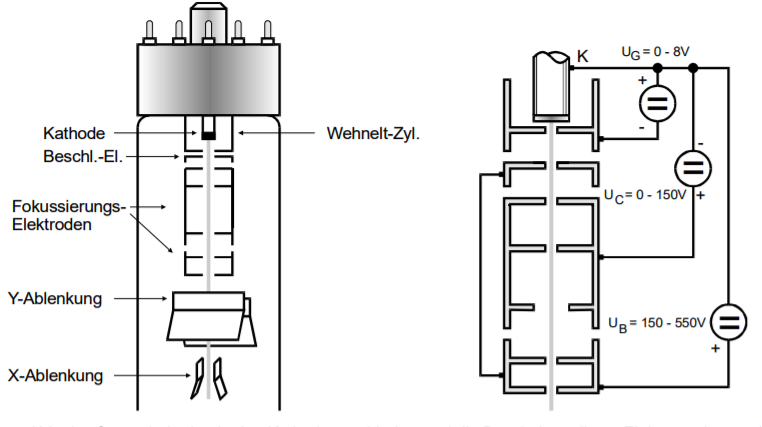
\includegraphics[height=8cm]{kathodenstrahlroehre.PNG}
  \caption{Aufbau einer Kathodenstrahlröhre(links) und Beschaltung einer Elektronenkanone (rechts)}
  \label{fig:kathode}
\end{figure}
